\documentclass{beamer}
\usepackage[utf8]{inputenc}
\usepackage[T1]{fontenc}
\usepackage{mathabx}
\usepackage{mathpazo}
\usepackage{eulervm}
\usepackage{natbib}
\usepackage{enumerate}
\usepackage{mathrsfs}

\usetheme{Madrid}
\usefonttheme{structurebold}
\usecolortheme{dove}
\title{VE401 Mid RC Pt.2}
\author{Wang Yangyang}
\date{2022 Spring}
\institute{UM-SJTU JI}
\setbeamersize{text margin left = 20pt, text margin right = 20pt}

\AtEndDocument{\begin{frame}{End}

                  Credit to Zhanpeng Zhou (TA of SP21)
                  
                  Credit to Fan Zhang (TA of SU21)
                  
                  Credit to Jiawen Fan (TA of SP21)
                  
                  Credit to Zhenghao Gu (TA of SP20)
                  
                  \url{https://www.johndcook.com/blog/distribution_chart/}
               \end{frame}
                }
                
\definecolor{antiquefuchsia}{rgb}{0.57, 0.36, 0.51}
\newcommand{\bb}[1]{\textcolor{antiquefuchsia}{\textbf{\textit{#1}}}}

\begin{document}
\maketitle

\begin{frame}
\frametitle{Outline}
\tableofcontents
\end{frame}

%\AtBeginSection[ ]
%{
%\begin{frame}{Outline for \secname}
%	\tableofcontents[currentsection, hideothersubsections, %sectionstyle=show/show]
%\end{frame}
%}

\AtBeginSubsection[]{
  \frame<beamer>{ 
    \frametitle{Outline}   
    \tableofcontents[currentsection,currentsubsection] 
  }
}

\section{Continuous Random Variables}
\subsection{Basics}
\begin{frame}{Continuous Random Variable: Def. and PDF}
\begin{block}{Definition}
Let $S$ be a sample space. A \bb{continuous random variable} is a map $X: S \rightarrow \mathbb{R}$ together with a function $f_{X}: \mathbb{R} \rightarrow \mathbb{R}$ with the properties that
\begin{enumerate}
\item $f_{X}(x) \geq 0$ for all $x \in \mathbb{R}$ and
\item $\int_{-\infty}^{\infty} f_{X}(x) \mathrm{d} x=1$.
\end{enumerate}
The integral of $f_{X}$ is interpreted as the probability that $X$ assumes values $X$ in a given range, i.e.,
$$
P[a \leq X \leq b]=\int_{a}^{b} f_{X}(x) \mathrm{d} x
$$
The function $f_{X}$ is called the \bb{probability density function} of random variable $X$.
\end{block}
\end{frame}

\begin{frame}{Continuous Random Variable: CDF and Location}
\begin{block}{Definition}
Let $\left(X, f_{X}\right)$ be a continuous random variable. The \bb{cumulative distribution function} for $X$ is defined by $F_{X}: \mathbb{R} \rightarrow \mathbb{R}$,
$$
F_{X}(x):=P[X \leq x]=\int_{-\infty}^{x} f_{X}(y) \mathrm{d} y
$$
\end{block}
By the fundamental theorem of calculus, we can obtain the density function from $F_{X}$ by
$$
f_{X}(x)=F_{X}^{\prime}(x)
$$
\begin{block}{Definition}
\begin{itemize}
\item The \bb{median} $M_{X}$ is defined by $P\left[X \leq M_{X}\right]=0.5$.
\item The \bb{mean} is given by $\mathrm{E}[X]$.
\item The \bb{mode} $x_{0}$, is the location of the maximum of $f_{X}$.
\end{itemize}
\end{block}
\end{frame}

\begin{frame}{Expectation, Variance and Moments}
\begin{itemize}
\item Expectation.
$$
\mathrm{E}[X]:=\int_{\mathbb{R}} x \cdot f_{X}(x) \mathrm{d} x
$$
\item Variance.
$$
\operatorname{Var}[X]:=\mathrm{E}\left[(X-\mathrm{E}[X])^{2}\right]=\mathrm{E}\left[X^{2}\right]-\mathrm{E}[X]^{2}
$$
\item M.G.F.
$$
m_{X}(t)=\mathrm{E}\left[e^{t X}\right]=\int_{-\infty}^{\infty} e^{t x} f_{X}(x) \mathrm{d} x
$$
\end{itemize}
\bb{Note:} All previous properties about expectation, variance and M.G.F. hold
for continuous random variables.
\end{frame}

\subsection{Exponential, Gamma, Chi-Squared Distribution}
\begin{frame}{Connections}
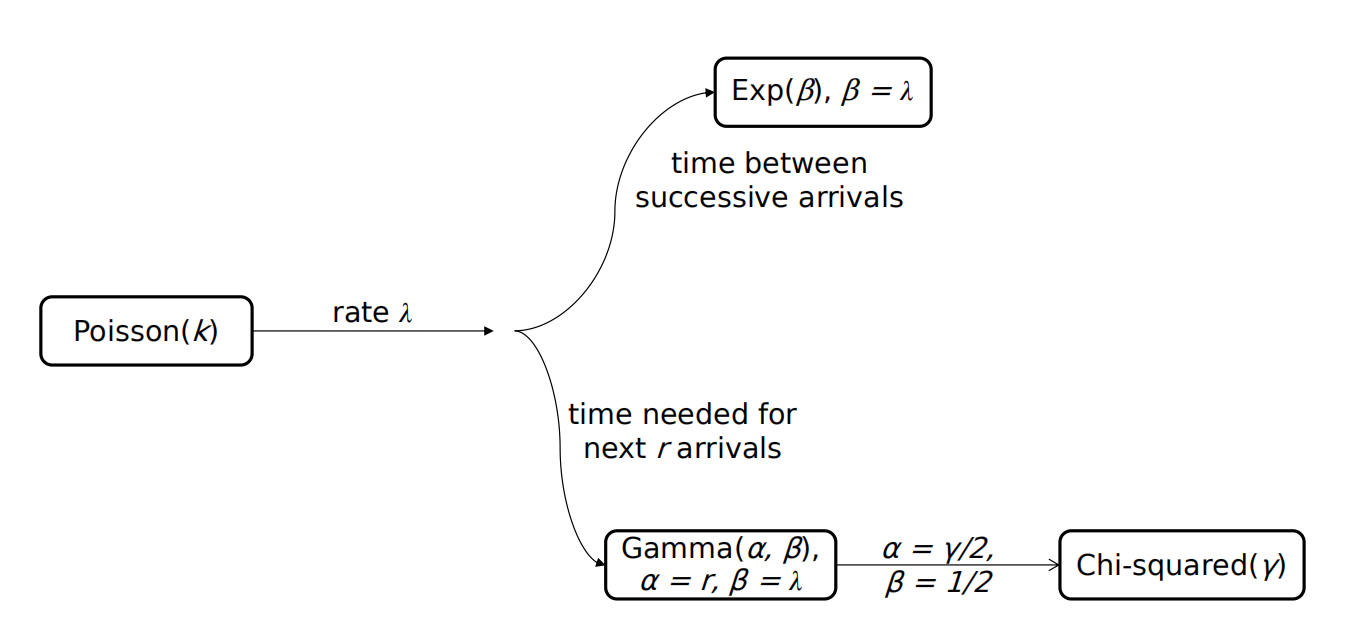
\includegraphics[scale=0.35]{connection.png}
\end{frame}

\begin{frame}{Exponential Distribution}
\begin{block}{Definition}
A continuous random variable $\left(X, f_{\beta}\right)$ follows \bb{exponential distribution} with parameter $\beta$ if the probability density function is defined by
$$
f_{\beta}(X)= \begin{cases}\beta e^{-\beta x}, & x>0 \\ 0, & x \leq 0\end{cases}
$$
\end{block}
\begin{block}{Interpretation}
The time between successive arrivals of a Poisson process with rate $\lambda$ follows exponential distribution with parameter $\beta=\lambda$. (Recall $\left.P[T>t]=e^{-\beta t} .\right)$
\bb{Note.} Memoryless property:
$$
P[X>x+s \mid X>x]=P[X>s]
$$
\end{block}
\end{frame}

\begin{frame}{Exponential Distribution}
\begin{block}{Properties}
\begin{itemize}
\item Mean.
$$
\mathrm{E}[X]=\frac{1}{\beta}
$$
\item Variance. 
$$
\operatorname{Var}[X]=\frac{1}{\beta^{2}}
$$
\item M.G.F.
$$
m_{X}:(-\infty, \beta) \rightarrow \mathbb{R}, \quad m_{X}(t)=\frac{1}{1-t / \beta}
$$
\end{itemize}
\end{block}
\end{frame}

\begin{frame}{Exponential Distribution}
\begin{block}{Plot}
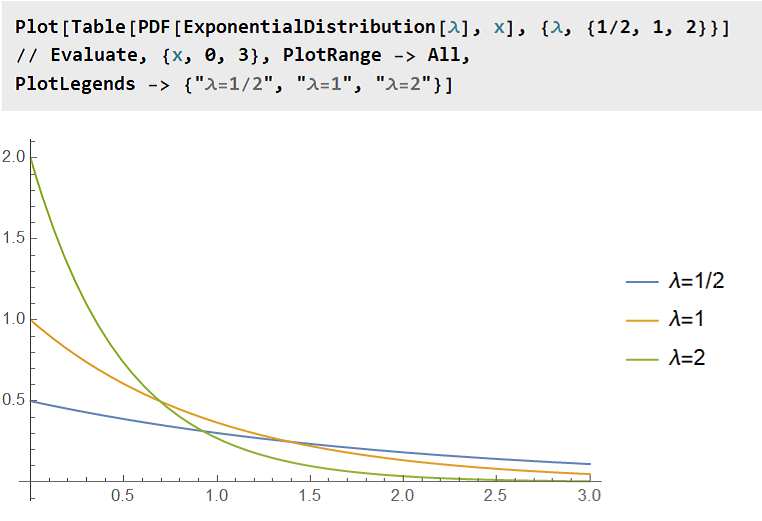
\includegraphics[scale=0.5]{plot.png}
\end{block}
\end{frame}


%%gamma
\begin{frame}{Gamma Distribution}
\begin{block}{Definition}
Let $\alpha, \beta \in \mathbb{R}, \alpha, \beta>0$. A continuous random variable $\left(X, f_{\alpha, \beta}\right)$ follows a gamma distribution with parameters $\alpha$ and $\beta$ if the probability density function is given by
$$
f_{\alpha, \beta}(x)= \begin{cases}\frac{\beta^{\alpha}}{\Gamma(\alpha)} x^{\alpha-1} e^{-\beta x}, & x>0 \\ 0, & x \leq 0\end{cases}
$$
\end{block}
where $\Gamma(\alpha)=\int_{0}^{\infty} z^{\alpha-1} e^{-z} \mathrm{~d} z, \alpha>0$ is the Euler gamma function.
Interpretation. 
\begin{block}{Interpretation}
The time needed for the next $r$ arrivals in a Poisson process with rate $\lambda$ follows a Gamma distribution with parameters $\alpha=r, \beta=\lambda$.
\end{block}
\end{frame}

\begin{frame}{Gamma Distribution}
\begin{block}{Properties}
\begin{itemize}
\item Mean.
$$
\mathrm{E}[X]=\frac{\alpha}{\beta}
$$
\item Variance. 
$$
\operatorname{Var}[X]=\frac{\alpha}{\beta^{2}}
$$
\item M.G.F.
$$
m_{X}:(-\infty, \beta) \rightarrow \mathbb{R}, \quad m_{X}(t)=\frac{1}{(1-t / \beta)^{\alpha}}
$$
\end{itemize}
\end{block}
\end{frame}


\begin{frame}{Gamma Distribution}
\begin{block}{Plot}
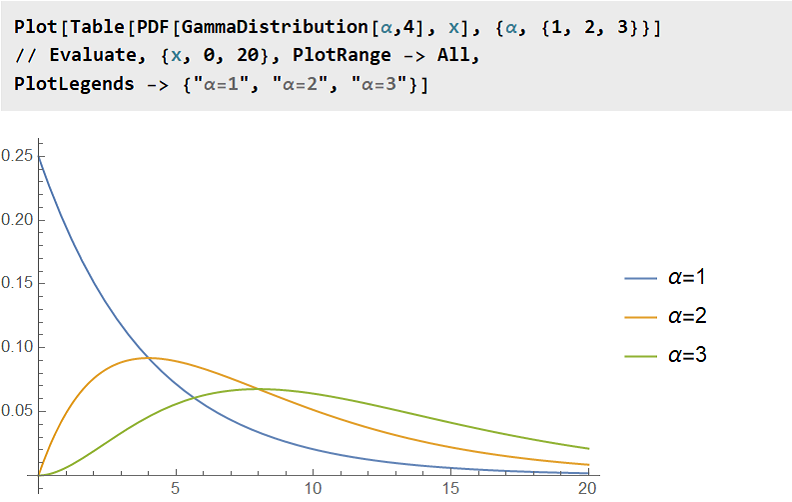
\includegraphics[scale=0.5]{gamma1.png}
\end{block}
\end{frame}

\begin{frame}{Gamma Distribution}
\begin{block}{Plot}
What's Wrong?
-- FOR $\beta$, MMA IS DIFFERENT FROM THE LECTURE! It's $(1/2,1/4,1/6)$ for the lecture version.

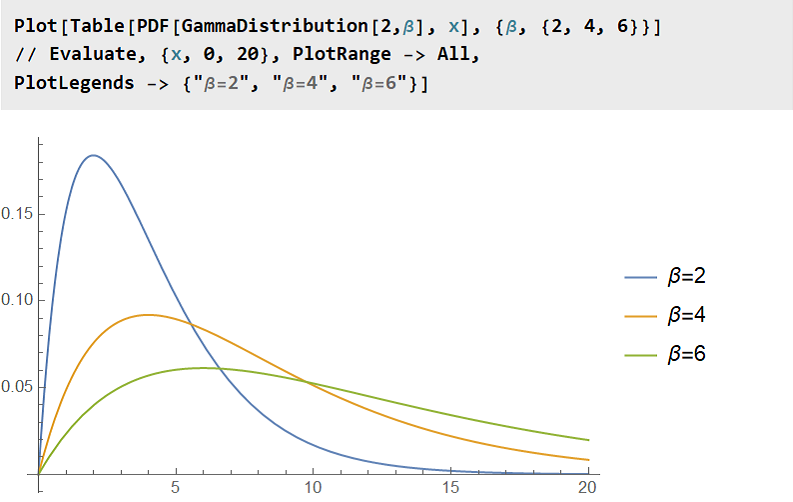
\includegraphics[scale=0.5]{gamma2.png}
\end{block}
\end{frame}

\begin{frame}{Chi-Squared Distribution}
\begin{block}{Definition}
Definition. Let $\gamma \in \mathbb{N}$. A continuous random variable $\left(X_{\gamma}^{2}, f_{X}\right)$ follows a chi-squared distribution with $\gamma$ degrees of freedom if the probability density function is given by
$$
f_{\gamma}(x)= \begin{cases}\frac{1}{2^{\gamma / 2} \Gamma(\gamma / 2)} x^{\gamma / 2-1} e^{-x / 2}, & x>0 \\ 0, & x \leq 0\end{cases}
$$
\end{block}
It is a gamma distribution with $\alpha=\gamma / 2, \beta=1 / 2$. Therefore,
$$
\mathrm{E}\left[X_{\gamma}^{2}\right]=\gamma, \quad \operatorname{Var}\left[X_{\gamma}^{2}\right]=2 \gamma
$$
\end{frame}

\begin{frame}{Chi-Squared Distribution}
\begin{block}{Plot}
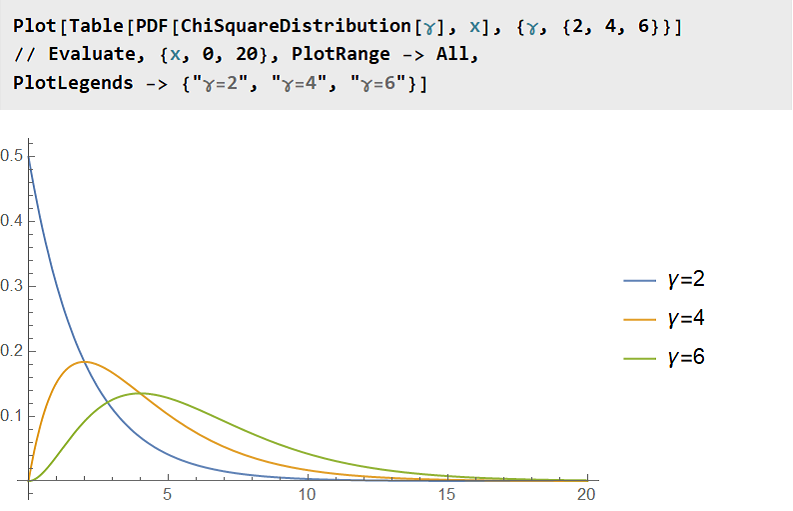
\includegraphics[scale=0.5]{chi.png}
\end{block}
\end{frame}

\subsection{Normal Distribution}
\begin{frame}{Normal Distribution}
\begin{block}{Definition}
A continuous random variable $\left(X, f_{\mu, \sigma^{2}}\right)$ has the \bb{normal distribution} with mean $\mu \in \mathbb{R}$ and variance $\sigma^{2}, \sigma>0$ if the probability density function is given by
$$
f_{\mu, \sigma^{2}}=\frac{1}{\sqrt{2 \pi \sigma^{2}}} \exp \left[-\frac{1}{2}\left(\frac{x-\mu}{\sigma}\right)^{2}\right], \quad x \in \mathbb{R}
$$
\end{block}
\begin{block}{Useful Formula}
Normal.
$$
\int_{-\infty}^{\infty} e^{-\frac{(x-\mu)^{2}}{2 \sigma^{2}}} d x=\sqrt{2 \pi} \sigma
$$
Gamma.
$$
\int_{0}^{\infty} x^{\alpha-1} e^{-\beta x} d x=\frac{\Gamma(\alpha)}{\beta^{\alpha}}
$$
\end{block}
\end{frame}

\begin{frame}{Normal Distribution}
\begin{block}{Properties}
\begin{itemize}
\item Mean.
$$
\mathrm{E}[X]=\mu
$$
\item Variance.
$$
\operatorname{Var}[X]=\sigma^{2}
$$
\item M.G.F.
$$
m_{X}: \mathbb{R} \rightarrow \mathbb{R}, \quad m_{X}(t)=\exp \left(\mu t+\frac{1}{2} \sigma^{2} t^{2}\right)
$$
\end{itemize}
\end{block} 
\end{frame}

\subsection{Transformation of R.V.}
\begin{frame}{Transformation of Random Variables}
\begin{block}{Theorem}
Let $X$ be a continuous random variable with density $f_{X}$. Let $Y=\varphi \circ X$, where $\varphi: \mathbb{R} \rightarrow \mathbb{R}$ is strictly \bb{monotonic and differentiable}. The density for $Y$ is then given by
$$f_{Y}(y)=f_{X}\left(\varphi^{-1}(y)\right) \cdot\left|\frac{\mathrm{d} \varphi^{-1}(y)}{\mathrm{d} y}\right|, \quad$$

for $y \in \operatorname{ran} \varphi$


and $$f_{Y}(y)=0, \quad$$ for $y \notin \operatorname{ran} \varphi .$
\end{block}
What if not \bb{monotonic and differentiable}? Consider \bb{CDF}.
\end{frame}



\begin{frame}{Transformation of Random Variables}
What if not \bb{monotonic and differentiable}? Consider \bb{CDF}.
\begin{block}{Example}
Consider the continuous random variable $X$ with density
$$
f_{X}(x)=\frac{2/\pi}{e^{-x}+e^{x}}
$$
for $x \in \mathbb{R}$

Find the density of the random variable $X^{2}$.
\end{block}
Things become easier using the observation that $f_X$ is an even function.
\end{frame}

\begin{frame}{Transformation of Random Variables}
\begin{block}{Solution}
Note that the function $\varphi: \mathbb{R} \rightarrow \mathbb{R}_{+} \cup\{0\}, \varphi(x)=x^{2}$ is not bijective, so we can't simply apply the theorem for transforming random variables from the lecture. Let $y>0$. Then, using the fact that $f_{X}$ is even,
$$
F_{Y}(y)=P[Y \leq y]=P\left[X^{2} \leq y\right]=P[-\sqrt{y} \leq X \leq \sqrt{y}]=\int_{-\sqrt{y}}^{\sqrt{y}} f_{X}(x) d x
$$
$$
\begin{aligned}
F_{Y}(y) &=P[Y \leq y]=P\left[X^{2} \leq y\right]=2 \int_{0}^{\sqrt{y}} f_{X}(x) d x
\end{aligned}
$$
$$
f_{Y}(y)=F_{Y}^{\prime}(y)=2 f_{X}(\sqrt{y}) \cdot \frac{1}{2 \sqrt{y}}=\frac{2}{\pi \sqrt{y}} \frac{1}{e^{-\sqrt{y}}+e^{\sqrt{y}}}\quad  y>0
$$
For $y \leq 0$ we have
$
F_{Y}(y)=P[Y \leq y]=P\left[X^{2} \leq y\right]=0,
$
so $$f_{Y}(y)=0 \quad y \leq 0 .$$
\end{block}
\end{frame}



\subsection{Standardizing and Normal Approximation}
\begin{frame}{Standardizing Normal Distribution}
Suppose $X \sim \operatorname{Normal}\left(\mu, \sigma^{2}\right) .$ Then
$$
Z=\frac{X-\mu}{\sigma} \sim \operatorname{Normal}(0,1)
$$
where the normal distribution with mean $\mu$ and variance $\sigma^{2}$ is the \bb{standard normal distribution}.

$\Phi$ is the cumulative distribution function for the standard normal distribution function.
$$
\Phi(z):=\frac{1}{\sqrt{2 \pi}} \int_{-\infty}^{z} e^{-t^{2} / 2} d t
$$
Calculate $P[X<a]$ by
$$
\begin{aligned}
P[X<a] &=P\left[\frac{X-\mu}{\sigma}<\frac{a-\mu}{\sigma}\right] =P\left[Z<\frac{a-\mu}{\sigma}\right] &=\Phi\left(\frac{a-\mu}{\sigma}\right)
\end{aligned}
$$
\end{frame}

\begin{frame}{Theorem of De Moivre-Laplace}
\begin{block}{Theorem}
Suppose $S_{n}$ is the number of successes in a sequence of $n$ i.i.d. Bernoulli trials with probability of success $0<p<1$. Then
$$
\lim _{n \rightarrow \infty} P\left[a<\frac{X-n p}{\sqrt{n p(1-p)}} \leq b\right]=\frac{1}{2 \pi} \int_{a}^{b} e^{-x^{2} / 2} \mathrm{~d} x
$$
\end{block}
\begin{center}
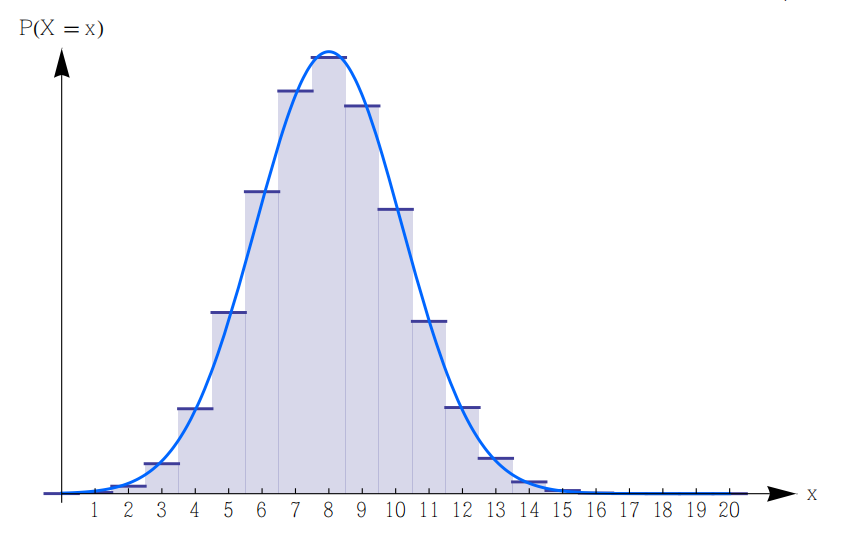
\includegraphics[scale=0.3]{appro.png}
\end{center}
\end{frame}

\begin{frame}{Normal Approximation of Binomial Distribution}
For $y=0, \ldots, n$
$$
P[X \leq y]=\sum_{x=0}^{y}\left(\begin{array}{l}
n \\
x
\end{array}\right) p^{x}(1-p)^{n-x} \approx \Phi\left(\frac{y+1 / 2-n p}{\sqrt{n p(1-p)}}\right)
$$
where we require that
$$
n p>5 \quad \text { if } p \leq \frac{1}{2} \quad \text { or } \quad n(1-p)>5 \quad \text { if } p>\frac{1}{2}
$$
This additional term $1 / 2$ is known as the \bb{half-unit correction} for the normal approximation to the \bb{cumulative} binomial distribution function.
\end{frame}

\subsection{Chebyshev's Inequality}
\begin{frame}{Chebyshev's Inequality and Law of Large Number}
\begin{block}{Theorem}
Let $X$ be a random variable, then for $k \in \mathbb{N} \backslash\{0\}$ and $c>0$,
$$
P[|X| \geq c] \leq \frac{\mathrm{E}\left[|X|^{k}\right]}{c^{k}}
$$
As another version of this inequality, suppose $X$ has mean $\mu$ and standard deviation $\sigma$, and let $m>0$,
$$
P[|X-\mu| \geq m \sigma] \leq \frac{1}{m^{2}}
$$
\end{block}
\begin{block}{Weak Law of Large Number}
Let $X_{1}, X_{2}, \ldots$ be a sequence of i.i.d. random variables with mean $\mu$ and variance $\sigma^{2}$. Then for any $\varepsilon>0$,
$$
P\left[\left|\frac{X_{1}+\ldots+X_{n}}{n}-\mu\right| \geq \varepsilon\right] \stackrel{n \rightarrow \infty}{\longrightarrow} 0
$$
\end{block}
\end{frame}

\begin{frame}{Central Limit Theorem}
\begin{block}{Theorem}
Central Limit Theorem. Let $\left(X_{i}\right)$ be a sequence of independent, but not necessarily identical random variables whose third moments exist and satisfy a certain technical condition. Let
$$
Y_{n}=X_{1}+\cdots+X_{n}
$$
Then for any $z \in \mathbb{R}$
$$
P\left[\frac{Y_{n}-\mathrm{E}\left[Y_{n}\right]}{\sqrt{\operatorname{Var}\left[Y_{n}\right]}} \leq z\right] \stackrel{n \rightarrow \infty}{\longrightarrow} \frac{1}{\sqrt{2 \pi}} \int_{-\infty}^{z} e^{-x^{2} / 2} d x
$$
\end{block}
\begin{block}{Interpretation}
Lyapunov’s Central Limit theorem is at the core of the belief by
experimentalists that “random error” may be described by the normal
distribution.
\end{block}
\end{frame}


\section{Multivariate Random Variables}
\subsection{Discrete, Continuous Multivariate R.V.}
\begin{frame}{Discrete Multivariate Random Variable}
\begin{block}{Definition}
Let $S$ be a sample space and $\Omega$ a countable subset of $\mathbb{R}^{n}$. A \bb{discrete multivariate random variable} is a map
$$
\mathbf{X}: S \rightarrow \Omega
$$
together with a function $f_{\mathbf{X}}: \Omega \rightarrow \mathbb{R}$ with the properties that
\begin{enumerate}
\item $f_{\mathbf{X}}(x) \geq 0$ for all $x=\left(x_{1}, \ldots, x_{n}\right) \in \Omega$ and
\item $\sum_{x \in \Omega} f_{\mathbf{X}}(x)=1$,
\end{enumerate}
where $f_{\mathbf{X}}$ is the \bb{joint density function} of the random variable $\mathbf{X}$.
\end{block}
\end{frame}

\begin{frame}{Continuous Multivariate Random Variable}
\begin{block}{Definition}
Let $S$ be a sample space. A \bb{continuous multivariate random variable} is a map
$$
\mathbf{X}: S \rightarrow \mathbb{R}^{n}
$$
together with a function $f_{\mathbf{X}}: \mathbb{R}^{n} \rightarrow \mathbb{R}$ with the properties that
\begin{enumerate}
\item $f_{\mathbf{X}}(x) \geq 0$ for all $x=\left(x_{1}, \ldots, x_{n}\right) \in \mathbb{R}^{n}$ and
\item $\int_{\mathbb{R}^{n}} f_{\mathbf{X}}(x)=1$,
\end{enumerate}
where $f_{\mathbf{X}}$ is the \bb{joint density function} of the random variable $\mathbf{X}$.
\end{block}
\end{frame}

\begin{frame}{Multivariate Random Variable}
\begin{itemize}
\item \bb{Marginal density} $f_{X_{k}}$ for $X_{k}, k=1, \ldots, n$ :
$$
f_{X_{k}}\left(x_{k}\right)=\int_{\mathbb{R}^{n-1}} f_{X}\left(x_{1}, \ldots, x_{n}\right) \mathrm{d} x_{1} \ldots \mathrm{d} x_{k-1} \mathrm{~d} x_{k+1} \ldots \mathrm{d} x_{n} .
$$
\item \bb{Independent} multivariate random variables:
$$
f_{X}\left(x_{1}, \ldots, x_{n}\right)=f_{X_{1}}\left(x_{1}\right) \cdots f_{X_{n}}\left(x_{n}\right) .
$$
\item \bb{Conditional density} of $X_{1}$ conditioned on $X_{2}$ :
$$
f_{X_{1} \mid X_{2}}\left(x_{1}\right):=\frac{f_{X_{1} X_{2}}\left(x_{1}, x_{2}\right)}{f_{X_{2}}\left(x_{2}\right)} \quad \text { whenever } f_{X_{2}}\left(x_{2}\right)>0 \text {. }
$$
\item \bb{Joint cumulative distribution function} (CDF) is then given by
$$
P\left[X_{1} \leq a_{1}, \ldots, X_{n} \leq a_{n}\right]=\int_{-\infty}^{a_{1}} \cdots \int_{-\infty}^{a_{n}} f_{X}(x) \mathrm{d} x_{1} \ldots \mathrm{d} x_{n}
$$
\end{itemize}
\end{frame}



\begin{frame}{Continuous Multivariate Random Variable}
\begin{block}{Visualization}
Joint probability density function $f_{X Y}(x, y)$ (left)

conditional density function $f_{X \mid Y}\left(x \mid y_{0}\right)$ (right).
\begin{center}
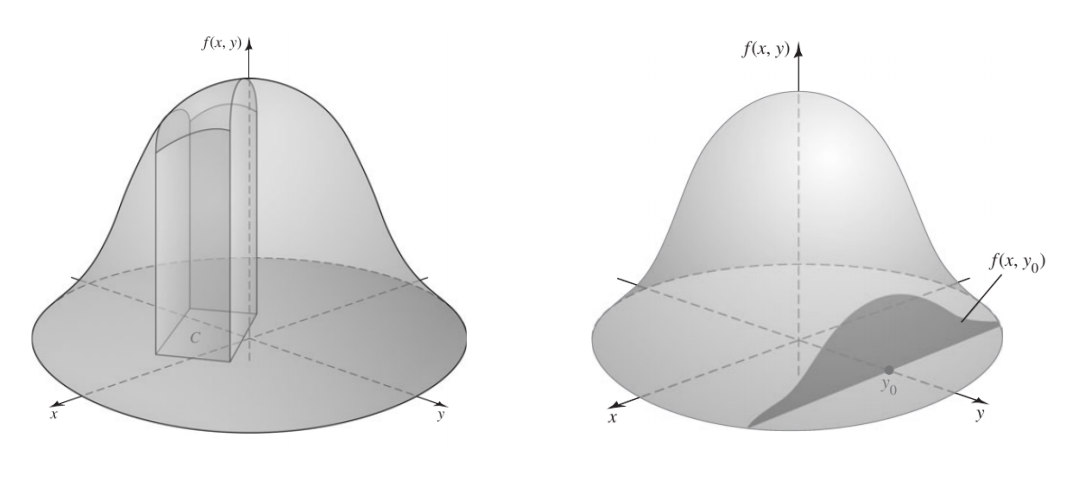
\includegraphics[scale=0.4]{vis.png}
\end{center}
\end{block}
\end{frame}



\subsection{Covariance and Correlation}
\begin{frame}{Expectation}
\begin{itemize}
\item Discrete.
$$
\mathrm{E}\left[X_{k}\right]=\sum_{x_{k}} x_{k} f_{X_{k}}\left(x_{k}\right)=\sum_{x \in \Omega} x_{k} f_{X}(x)
$$
and for continuous function $\varphi: \mathbb{R}^{n} \rightarrow \mathbb{R}$,
$$
\mathrm{E}[\varphi \circ \mathbf{X}]=\sum_{x \in \Omega} \varphi(x) f_{\mathbf{X}}(x)
$$
\item Continuous.
$$
\mathrm{E}\left[X_{k}\right]=\int_{\mathbb{R}} x_{k} f_{X_{k}}\left(x_{k}\right) \mathrm{d} x_{k}=\int_{\mathbb{R}^{n}} x_{k} f_{X}(x) \mathrm{d} x
$$
and for continuous function $\varphi: \mathbb{R}^{n} \rightarrow \mathbb{R}$,
$$
\mathrm{E}[\varphi \circ \mathbf{X}]=\int_{\mathbb{R}^{n}} \varphi(x) f_{\mathbf{X}}(x) \mathrm{d} x .
$$
\end{itemize}
\end{frame}


\begin{frame}{Covariance}
\begin{block}{Definition}
Definition. For a multivariate random variable $\mathbf{X}$, the \bb{covariance matrix} $\operatorname{Var}[\mathbf{X}]$ is given by
$$
\left(\begin{array}{cccc}
\operatorname{Var}\left[X_{1}\right] & \operatorname{Cov}\left[X_{1}, X_{2}\right] & \cdots & \operatorname{Cov}\left[X_{1}, X_{n}\right] \\
\operatorname{Cov}\left[X_{1}, X_{2}\right] & \operatorname{Var}\left[X_{2}\right] & \ddots & \vdots \\
\vdots & \ddots & \ddots & \operatorname{Cov}\left[X_{n-1}, X_{n}\right] \\
\operatorname{Cov}\left[X_{1}, X_{n}\right] & \cdots & \operatorname{Cov}\left[X_{n-1}, X_{n}\right] & \operatorname{Var}\left[X_{n}\right]
\end{array}\right)
$$
where the \bb{covariance} of $\left(X_{i}, X_{j}\right)$ is given by
$$
\operatorname{Cov}\left[X_{i}, X_{j}\right]=\mathrm{E}\left[\left(X_{i}-\mu_{X_{i}}\right)\left(X_{j}-\mu_{X_{j}}\right)\right]=\mathrm{E}\left[X_{i} X_{j}\right]-\mathrm{E}\left[X_{i}\right] \mathrm{E}\left[X_{j}\right]
$$
and
$$
\operatorname{Var}[\mathbf{C X}]=\mathbf{C} \operatorname{Var}[\mathbf{X}] \mathbf{C}^{T}, \quad \mathbf{C} \in \operatorname{Mat}(n \times n ; \mathbb{R})
$$
\end{block}
\end{frame}

\begin{frame}{Covariance}
\begin{block}{Properties}
Let $X, X_{1}, \ldots, X_{n}, Y$ and $Z$ be random variables.
\begin{itemize}
\item $X$ and $Y$ are independent $\Rightarrow \operatorname{Cov}[X, Y]=0$.

The Converse is not True!

\item $\operatorname{Var}[X+Y]=\operatorname{Var}[X]+\operatorname{Var}[Y]+2 \operatorname{Cov}[X, Y]$, and more generally,
$$
\begin{aligned}
\operatorname{Var}\left[X_{1}+\cdots+X_{n}\right]=\operatorname{Var}\left[X_{1}\right]+\cdots+& \operatorname{Var}\left[X_{n}\right]+2 \sum_{i<j} \operatorname{Cov}\left[X_{i}, X_{j}\right]
\end{aligned}
$$
if $\operatorname{Var}\left[X_{i}\right]<\infty$ for $i=1, \ldots, n$
\item $\operatorname{Cov}[X, Y+Z] = \operatorname{Cov}[X, Y] + \operatorname{Cov}[X, Z]$ 

$\operatorname{Cov}[X, Y-Z] = \operatorname{Cov}[X, Y] - \operatorname{Cov}[X, Z]$
\item $\operatorname{Cov}[X, X] = \operatorname{Var}[X]$
\end{itemize}
\end{block}
\end{frame}

\begin{frame}{Correlation}
\begin{block}{Definition}
The \bb{Pearson coefficient of correlation} of random variables $X$ and $Y$ is given by
$$
\rho_{X Y}:=\frac{\operatorname{Cov}[X, Y]}{\sqrt{\operatorname{Var}[X] \operatorname{Var}[Y]}}
$$
\end{block}
Instead of independence, the correlation coefficient actually measures the the extent to which $X$ and $Y$ are \bb{linearly} dependent, which is not the only way of being dependent.
\begin{block}{Properties}
\begin{itemize}
\item $-1 \leq \rho_{X Y} \leq 1$,
\item $\left|\rho_{X Y}\right|=1$ iff there exist $\beta_{0}, \beta_{1} \in \mathbb{R}$ such that
$$
Y=\beta_{0}+\beta_{1} X
$$
\end{itemize}
\end{block}
\end{frame}

\begin{frame}{Correlation}
\begin{block}{Note}
\begin{itemize}
\item Uncorrelated does not mean independent,
\item Correlation coefficient only measures linear relationships.
\end{itemize}
\end{block}
\begin{block}{Example}
Two random variables $X$ and $Y . X$ follows a uniform distribution $U(-1,1)$ and $Y=X^{2}$. Find $\operatorname{Cov}(X, Y)$.
$$
\begin{aligned}
\operatorname{Cov}(X, Y) &=\operatorname{Cov}\left(X, X^{2}\right) \\
&=\mathrm{E}\left((X-\mathrm{E}(X))\left(X^{2}-\mathrm{E}\left(X^{2}\right)\right)\right) \\
&=\mathrm{E}\left(X^{3}-X^{2} \mathrm{E}(X)-X \mathrm{E}\left(X^{2}\right)+\mathrm{E}(X) \mathrm{E}\left(X^{2}\right)\right) \\
&=\mathrm{E}\left(X^{3}\right)-\mathrm{E}\left(X^{2}\right) \mathrm{E}(X)-\mathrm{E}(X) \mathrm{E}\left(X^{2}\right)+\mathrm{E}(X) \mathrm{E}\left(X^{2}\right) \\
&=\int_{-1}^{1} \frac{1}{2} x^{3} \mathrm{~d} x-\int_{-1}^{1} \frac{1}{2} x^{2} \mathrm{~d} x \cdot \int_{-1}^{1} \frac{1}{2} x \mathrm{~d} x =0
\end{aligned}
$$
\end{block}
\end{frame}

\begin{frame}{The Fisher Transformation}
\begin{block}{Definition}
Let $\widetilde{X}$ and $\widetilde{Y}$ be standardized random variables of $X$ and $Y$, then the \bb{Fisher transformation} of $\rho_{X Y}$ is given by
$$\ln \left(\sqrt{\frac{\operatorname{Var}[\widetilde{X}+\widetilde{Y}]}{\operatorname{Var}[\widetilde{X}-\widetilde{Y}]}}\right)=\frac{1}{2} \ln \left(\frac{1+\rho_{X Y}}{1-\rho_{X Y}}\right)=\operatorname{Arctanh}\left(\rho_{X Y}\right) \in \mathbb{R}$$
We say that $X$ and $Y$ are
\begin{itemize}
\item \bb{positively correlated} if $\rho_{X Y}>0$, and
\item \bb{negatively correlated} if $\rho_{X Y}<0$.
\end{itemize}
\end{block}
\end{frame}

\begin{frame}{The Bivariate Normal Distribution}
The density function of \bb{Bivariate Normal Distribution}:
$$
f_{X Y}(x, y)=\frac{1}{2 \pi \sigma_{X} \sigma_{Y} \sqrt{1-\varrho^{2}}} e^{-\frac{1}{2\left(1-\varrho^{2}\right)}\left[\left(\frac{x-\mu_{X}}{\sigma_{X}}\right)^{2}-2 \varrho\left(\frac{x-\mu_{X}}{\sigma_{X}}\right)\left(\frac{y-\mu_{Y}}{\sigma_{Y}}\right)+\left(\frac{y-\mu_{Y}}{\sigma_{Y}}\right)^{2}\right]}
$$
\begin{itemize}
\item $-1<\varrho<1$
\item $\mu_{X}=\mathrm{E}[X], \sigma_{X}^{2}=\operatorname{Var} X$ (and similarly for $Y$ ).
\item $\varrho=\rho_{X Y}$ is indeed the correlation coefficient of $X$ and $Y$.
\item $X$ and $Y$ are independent $\Longleftrightarrow \varrho=0$
\end{itemize}
\end{frame}

\subsection{Hypergeometric Distribution}
\begin{frame}{Hypergeometric Distribution}
\begin{block}{Definition}
A random variable $\left(X, f_{X}\right)$ with parameters $N, n, r \in \mathbb{N} \backslash\{0\}$ where $r, n \leq N$ and $n<\min \{r, N-r\}$ has a \bb{hypergeometric distribution} if the density function is given by
$$
f_{X}(x)=\frac{\left(\begin{array}{l}
r \\
x
\end{array}\right)\left(\begin{array}{l}
N-r \\
n-x
\end{array}\right)}{\left(\begin{array}{l}
N \\
n
\end{array}\right)}
$$

\end{block}
\begin{block}{Interpretation}
\begin{itemize}
\item $f_{X}(x)$ is the probability of getting $x$ red balls in drawing $n$ balls from a box containing $N$ balls, where $r$ of them are red.
\item This can be formulated as obtaining $x$ successes in $n$ identical but not independent Bernoulli trials, each with probability of success $\frac{r}{N}$.
\end{itemize}
\end{block}
\end{frame}

\begin{frame}{Hypergeometric Distribution}
\begin{block}{Property}
\begin{itemize}
\item Expectation
$$
\mathrm{E}[X]=\mathrm{E}\left[X_{1}+\cdots+X_{n}\right]=n \frac{r}{N}
$$
\item Variance
$$
\begin{aligned}
\operatorname{Var}[X] &=\operatorname{Var}\left[X_{1}+\cdots+X_{n}\right] \\
&=\operatorname{Var}\left[X_{1}\right]+\cdots+\operatorname{Var}\left[X_{n}\right]+2 \sum_{i<j} \operatorname{Cov}\left[X_{i}, X_{j}\right] \\
&=n \frac{r}{N} \frac{N-r}{N} \frac{N-n}{N-1}
\end{aligned}
$$
\end{itemize}
The \bb{binomial distribution} may be used to approximate the hypergeometric distribution if $n / N$ is small (less than $0.05$).
\end{block}
\end{frame}

\subsection{Transformation of R.V. and Application}
\begin{frame}{Transformation of Random Variables}
\begin{block}{Theorem}
Let $\left(\boldsymbol{X}, f_{\boldsymbol{X}}\right)$ be a continuous multivariate random variable and let $\varphi: \mathbb{R}^{n} \rightarrow \mathbb{R}^{n}$ be a differentiable, bijective map with inverse $\varphi^{-1}$. Then $\boldsymbol{Y}=\varphi \circ \boldsymbol{X}$ is a continuous multivariate random variable with density
$$
f_{Y}(y)=f_{X} \circ \varphi^{-1}(y) \cdot\left|\operatorname{det} D \varphi^{-1}(y)\right|,
$$
where $D \varphi^{-1}$ is the Jacobian of $\varphi^{-1}$.
\end{block}
\begin{itemize}
\item $f_{Y}(y)=0$ for $y \notin \operatorname{ran} \varphi$.
\end{itemize}
\end{frame}

\begin{frame}{Quotient of Normal: Cauchy}
\begin{block}{Lemma}
Let $\left((X, Y), f_{X Y}\right)$ be a continuous bivariate random variable. Let $U=X / Y$. Then the density $f_{U}$ of $U$ is given by
$$
f_{U}(u)=\int_{-\infty}^{\infty} f_{X Y}(u v, v) \cdot|v| d v .
$$
\end{block}
\begin{block}{Theorem}
Suppose that random variables $X$ and $Y$ are independent and that each follows the \bb{standard normal distribution}. Then $U=X / Y$ has the \bb{Cauchy distribution} with probability density function given by
$$
f_{U}(u)=\frac{1}{\pi\left(1+u^{2}\right)}, \quad u \in \mathbb{R} .
$$
\end{block}
\end{frame}

\begin{frame}{Quotient of Normal: Cauchy}
\begin{block}{Proof}
Let $V=Y$, excluding $Y=0$, the transformation from $(X, Y)$ to $(U, V)$ is one-to-one. Then $X=U V, Y=V$ and
$$
J=\operatorname{det}\left(\begin{array}{ll}
\frac{\partial x}{\partial u} & \frac{\partial x}{\partial v} \\
\frac{\partial y}{\partial u} & \frac{\partial y}{\partial v}
\end{array}\right)=v
$$
Then the joint density function is given by
$$
f_{U V}(u, v)=f_{X Y}(u v, v)|v|=\frac{|v|}{2 \pi} \exp \left(-\frac{1}{2}\left(u^{2}+1\right) v^{2}\right)
$$
Then the marginal of $U$ is calculated as
$$
f_{U}(u)=\int_{-\infty}^{\infty} f_{U v}(u, v) \mathrm{d} v=\frac{1}{\pi\left(u^{2}+1\right)}, \quad u \in \mathbb{R} .
$$
\end{block}
\end{frame}

\begin{frame}{Root Sum of Normal Square: Chi}
\begin{block}{Definition}
$\chi_{n}$ is a \bb{chi random variable} with $n$ \bb{degrees of freedom},
$$
\chi_{n}=\sqrt{\sum_{i=1}^{n} Z_{i}^{2}}
$$
where $Z_{1}, \ldots, Z_{n}$ are \bb{independent standard normal} random variables. 
$$f_{\chi_{n}}(y)=\frac{1}{2^{n / 2} \Gamma\left(\frac{n}{2}\right)} y^{n-1} e^{-y^2 / 2}\quad (y>0)$$
\end{block}

\begin{block}{Interpretation}
A chi random variable represents the sum of the root squares (distance) of independent standard normal variables.
\end{block}
\end{frame}



\begin{frame}{Sum of Normal Square: Chi-Squared}
\begin{block}{Definition}
$\chi_{n}^2$ is a \bb{chi-squared random variable} with $n$ \bb{degrees of freedom},
$$
\chi_{n}^{2}=\sum_{i=1}^{n} Z_{i}^{2}
$$
where $Z_{1}, \ldots, Z_{n}$ are \bb{independent standard normal} random variables. 
$$f_{\chi_{n}^{2}}(y)=\frac{1}{2^{n / 2} \Gamma\left(\frac{n}{2}\right)} y^{n / 2-1} e^{-y / 2}\quad (y>0)$$
\end{block}

\begin{block}{Interpretation}
A chi-squared random variable represents the sum of the squares of independent standard normal variables.
\end{block}
\end{frame}

\begin{frame}{Sum of Normal: Normal}
\begin{block}{Theorem}
If the random variables $X_{1}, \ldots, X_{k}$ are independent and if $X_{i}$ follows \bb{normal distribution} with mean $\mu_{i}$ and variance $\sigma_{i}^{2}$, where $i=1, \ldots, k$, then
$
X=X_{1}+\cdots+X_{k}
$
follows normal distribution with
$$
\mu=\mu_{1}+\cdots+\mu_{k}, \quad \sigma^{2}=\sigma_{1}^{2}+\cdots+\sigma_{k}^{2} .
$$
\end{block}
\begin{block}{Theorem}
Let $\chi_{\gamma_{1}}^{2}, \ldots, \chi_{\gamma_{n}}^{2}$ be $n$ independent random variables following \bb{chi-squared distributions} with $\gamma_{1}, \ldots, \gamma_{n}$ degrees of freedom, respectively. Then
$$
\chi_{\alpha}^{2}:=\sum_{k=1}^{n} \chi_{\gamma_{k}}^{2}
$$
is a \bb{chi-squared random variable} with $\alpha=\sum_{k=1}^{n} \gamma_{k}$ degrees of freedom.
\end{block}
\end{frame}

\section{Reliability}
\subsection{Reliability and Hazard}
\begin{frame}{Reliability}
\begin{block}{Definition}
Suppose a unit $A$ fails \bb{randomly}, and we describe the time it fails by the continuous random variable $T_{A}$.

The density of $T_{A}$ is called the \bb{failure density} $f_{A}$.
The cumulative distribution function of $T_{A}$ is denoted by $F_{A}$.
We note that
$$
\begin{aligned}
f_{A}(t) &=\lim _{\Delta t \rightarrow 0} \frac{P[t \leq T \leq t+\Delta t]}{\Delta t} \\
&=\lim _{\Delta t \rightarrow 0} \frac{F_{A}(t+\Delta t)-F_{A}(t)}{\Delta t}
\end{aligned}
$$

The \bb{reliability function} $R_{A}$ gives the probability that $A$ is working at time $t \geq 0$
$$
\begin{aligned}
R_{A}(0) &=1 \\
R_{A}(t) &=1-P[\text { component A fails before time } t] \\
&=1-F_{A}(t)
\end{aligned}
$$
\end{block}
\end{frame}

\begin{frame}{Hazard}
\begin{block}{Definition}
\bb{Hazard rate} $\varrho_{A}$ defined by
$$
\begin{aligned}
\varrho_{A}(t) &=\lim _{\Delta t \rightarrow 0} \frac{P[t \leq T \leq t+\Delta t \mid t \leq T]}{\Delta t} \\
&=\lim _{\Delta t \rightarrow 0} \frac{P[t \leq T \leq t+\Delta t]}{P[T \geq t] \cdot \Delta t}=\frac{f_{A}(t)}{R_{A}(t)}
\end{aligned}
$$
\end{block}
\begin{block}{Interpretation}
\begin{itemize}
\item If $\varrho$ is decreasing, then as time goes by a failure is more likely to occur earlier in the time interval.
\item If $\varrho$ is steady, a failure tends to occur during this period due mainly to random factors.
\item If $\varrho$ is increasing, then as time goes by a failure is more likely to occur.
\end{itemize}
\end{block}
\end{frame}


\subsection{Distribution and System}
\begin{frame}{Exponential Distribution}
\begin{itemize}
\item Density function. $\beta>0$ is a parameter,
$$
f(x)= \begin{cases}\beta e^{-\beta x}, & x>0 \\ 0, & \text { otherwise. }\end{cases}
$$
\item Mean.
$$
\mu=\frac{1}{\beta}
$$
\item Variance.
$$
\sigma^{2}=\frac{1}{\beta^{2}}
$$
\item Reliability features.
$$
\rho(t)=\beta$$$$R(t)=e^{-\beta t}, f(t)=\rho(t) R(t)=\beta e^{-\beta t} .
$$
\end{itemize}
\end{frame}

\begin{frame}{Weibull Distribution}
\begin{itemize}
\item Density function. $\alpha, \beta>0$ are parameters,
$$
f(x)= \begin{cases}\alpha \beta x^{\beta-1} e^{-\alpha x^{\beta}}, & x>0 \\ 0, & \text { otherwise }\end{cases}
$$
\item Mean.
$$
\mu=\alpha^{-1 / \beta} \Gamma(1+1 / \beta)
$$
\item Variance.
$$
\sigma^{2}=\alpha^{-2 / \beta} \Gamma(1+2 / \beta)-\mu^{2}
$$
\item Reliability features.
$$
\rho(t)=\alpha \beta t^{\beta-1}$$$$ R(t)=e^{-\alpha t^{\beta}}, f(t)=\rho(t) R(t)=\alpha \beta t^{\beta-1} e^{-\alpha t^{\beta}}
$$
\end{itemize}
\end{frame}

\begin{frame}{System}
$R_{i}$ is the reliability of the ith component, then
\begin{enumerate}
\item reliability of a series system with $k$ components
$$
R_{s}(t)=\prod_{i=1}^{k} R_{i}(t)
$$
\item reliability of a parallel system with $k$ components
$$R_{p}(t)=1-P\text{[all components fail before t]}=1-\prod_{i=1}^{k}\left(1-R_{i}(t)\right)$$
\end{enumerate}
\end{frame}


\end{document}
%%Hyper变example,加一个CDF transform example,第三第四题